\documentclass[12pt]{article}
\usepackage{amsmath}
\usepackage{graphicx}
\usepackage{pslatex}  % nice fonts
\usepackage{url} % for URLs

% page dimensions
\textwidth=6.5in
\oddsidemargin=-0.0in
\evensidemargin=-0.0in
\topmargin=-0.5in
\footskip=0.8in
\textheight=8.50in


% list shortcuts
\newcommand{\enum}[1]{\begin{enumerate} #1 \end{enumerate}}
\newcommand{\items}[1]{\begin{itemize} #1 \end{itemize}}

% formatting macros
\newcommand{\bold}[1]{{\bf #1}}
\newcommand{\ul}[1]{\underline{#1}}
\newcommand{\code}[1]{{\tt #1}}
\newcommand{\codeblock}[1]{\vspace{.1in} {\tt #1} \vspace{.1in}}

% reference macros
\newcommand{\figref}[1]{Figure~\ref{#1}}
\newcommand{\secref}[1]{Section~\ref{#1}}
\newcommand{\algref}[1]{Algorithm~\ref{#1}}

\newcommand{\comment}[1]{}

\newcommand{\version}{1.8.5}


% TODO: add development documentation

%%%%%%%%%%%%%%%%%%%%%%%%%%%%%%%%%%%%%%%%%%%%%%%%%%%%%%%%%%%%%%%%%%%%%%%%%%%%

\begin{document}

\begin{titlepage}

\begin{center}

\vspace*{2.5in}

{\huge \bf \fontfamily{phv}\selectfont 
SUMMON \version\ Manual
}
\vspace*{.5in}

{\large
Matt Rasmussen

\today
}
\vspace*{.5in}

Computer Science and Artificial Intelligence Lab

Massachusetts Institute of Technology

\vspace*{.25in}

rasmus@mit.edu
\end{center}

\end{titlepage}


\tableofcontents

\clearpage

%%%%%%%%%%%%%%%%%%%%%%%%%%%%%%%%%%%%%%%%%%%%%%%%%%%%%%%%%%%%%%%%%%%%%%%%%%%%
\section{Introduction}
\label{sec:intro}


\subsection{What is SUMMON}

SUMMON is a python extension module that provides rapid prototyping of 2D
visualizations.  By heavily relying on the python scripting language, SUMMON
allows the user to rapidly prototype a custom visualization for their data, 
without the overhead of a designing a graphical user interface or recompiling 
native code.  By simplifying the task of designing a visualization, users can 
spend more time on understanding their data. 

SUMMON was designed with several philosophies.  First, recompilation should
be avoided in order to speed up the development process.  Second, design of
graphical user interfaces should also be minimized.  Designing a good interface
takes planning and time to layout buttons, scrollbars, and dialog boxes.  Yet a 
poor interface is very painful to work with. Even when one has a good interface,
rarely can it be automated for batch mode.  Instead, SUMMON relies on the python
terminal for most interaction.  This allows the users direct access to  the
underlining code, which is more expressive, and can be automated through
scripting.  

Lastly, SUMMON is designed to be fast.  Libraries already exist for
accessing OpenGL in python.  However, python is relatively slow for real-time
interaction with large visualizations (trees with 100,000 leaves, matrices with
a million non-zeros, etc.).  Therefore, all real-time interaction is handled
with compiled native C++ code.  Python is only executed in the construction 
and occasional interaction with the visualization.  This arrangement provides 
the best of both worlds.




\subsection{Features}

Listed below is a short summary of the features offered in this version of
SUMMON.

\items{
    \item Python module extension
    \item Fast OpenGL graphics
    \item Drawing arbitrary points, lines, polygons, text with python scripting
    \item Binding inputs (keyboard, mouse, hotspots) to any python function 
    \item Separate threads for python and graphics (allows use of python prompt
          and responsive graphic at the same time)    
    \item Transparently handles graphics event loop, scrolling, zooming, text
          layout (auto-clipping, scaling, alignment), detecting clicks, allowing
          you to focus on viewing your data
    \item SVG output (also GIF/PNG/JPG/etc with ImageMagick)
    \item cross-platform (windows, linux)
}


%%%%%%%%%%%%%%%%%%%%%%%%%%%%%%%%%%%%%%%%%%%%%%%%%%%%%%%%%%%%%%%%%%%%%%%%%%%%
\section{Installing SUMMON}
\label{sec:installing}

The latest version of SUMMON can be obtained from 
http://people.csail.mit.edu/rasmus/summon/.  Download the *.tar.gz archive and
unzip it with the command:

\codeblock{tar zxvf summon-\version.tar.gz}

Before running or compiling SUMMON, the following libraries are required:
\items {
    \item python 2.4 (or greater)
    \item GL   
    \item GLUT
    \item SDL (for threading)
}

\subsection{Compiling SUMMON}

It is recommend to install SUMMON using the standard distutils 
(http://docs.python.org/inst/inst.html).  For example, in the
\code{summon-\version} directory run:

\codeblock{python setup.py install}

To install SUMMON in another location other than in \code{/usr} use:

\codeblock{python setup.py install --prefix=<another directory prefix>}

For more information and other install options see 
\code{summon-\version/INSTALL}.


\subsection{Configuring SUMMON}

SUMMON expects to find a configuration file called  \code{summon\_config.py}
somewhere in the python path.  Distutils installs a default module located in
your python path.  To customize SUMMON with your own key bindings and behavior,
you can write your own \code{summon\_config.py} file.  Just be sure it appears
in your python path somewhere {\em before} SUMMON default configuration file. 
Alternatively, you can create a configuration file \code{.summon\_config} in
your home directory.  The configuration file is nothing more than a python
script that calls the SUMMON function  \code{set\_binding} in order to
initialize the default keyboard and mouse  bindings.



%%%%%%%%%%%%%%%%%%%%%%%%%%%%%%%%%%%%%%%%%%%%%%%%%%%%%%%%%%%%%%%%%%%%%%%%%%%%
\section{Using SUMMON}
\label{sec:using}

SUMMON can be used as stand-alone program and as a module in a larger python
program.  The stand-alone version is installed in \code{PREFIX/bin/summon} and
is called from the command line as follows:

\codeblock{usage: summon [python script]}

On execution, SUMMON opens an OpenGL window and evaluates any script that it is
given in the python engine. After evaluation, the SUMMON prompt should appear
which provides direct access to the python engine.  Users should be familiar
with the python language in order to use SUMMON.

The SUMMON prompt acts exactly like the python prompt except for the OpenGL
window and the appearance of several automatically imported modules such as 
\code{summon}.  All of the commands needed to interact with the visualization
are within the \code{summon}  module.  

To learn how to use SUMMON, example scripts have been provided in the 
\code{summon/examples/} directory.  Examples of full fledged visualizations,
SUMMATRIX and SUMTREE, are also given in the \code{summon/bin/} directory. 
Their example input files are given in \code{summon/examples/summatrix/} and
\code{summon/examples/sumtree/}, respectively.



\subsection{Example script}

For an introduction to the basic API of SUMMON, let us walk through the
code of the first example.  This example is included in the downloaded
source code under the \code{summon/examples} directory.  To begin, change into the
\code{summon/examples/} directory and open up \code{01\_basics.py} in a
text editor.  Also execute the example with following command.

\codeblock{python -i 01\_basics.py}

The visualization (\figref{fig:01_basics}) should immediately appear in your
OpenGL window.  See \figref{fig:bindings} for a full list of available 
mouse and key-bindings.


\begin{figure}
\begin{center}
\footnotesize
\begin{tabular}{ll}

    {\bf Scroll \& zoom}     & \\ \hline 
    left mouse button          & activate/click \\
    left mouse button drag     & scroll \\
    right mouse button         & zoom (down: zoom-out, up: zoom-in)\\
    \\
    
    {\bf More ways to scroll \& zoom}     & \\ \hline 
    Ctrl + right mouse button  & zoom x-axis (down: zoom-out, up: zoom-in)\\
    Shift + right mouse button & zoom y-axis (down: zoom-out, up: zoom-in)\\
    arrow keys                 & scroll \\
    Shift + arrow keys         & scroll faster \\
    Ctrl + up key              & zoom in \\
    Ctrl + down key            & zoom out \\
    Shift + up key             & zoom in (y-axis only) \\
    Shift + down key           & zoom out (y-axis only) \\
    Shift + right key          & zoom in (x-axis only) \\
    Shift + left key           & zoom out (x-axis only) \\
    \\
    
    {\bf Miscellaneous} & \\ \hline
    middle click               & display pop-up menu \\    
    h                          & home (zoom to make all graphics visible) \\
    Ctrl + h                   & zoom 1:1 (restore zoom to 1:1 for x- and y-axis) \\
    Ctrl + l                   & toggle anti-aliasing \\
    Ctrl + d                   & duplicate window \\
    Ctrl + p                   & output SVG of the current view \\
    Ctrl + Shift + p           & output PNG of the current view \\
    Ctrl + x                   & show/hide crosshair \\
    q                          & close window \\
\end{tabular}
\end{center}
\caption{Default mouse and key-bindings for any SUMMON window}
\label{fig:bindings}
\end{figure}

%============================
\begin{figure}
\begin{center}
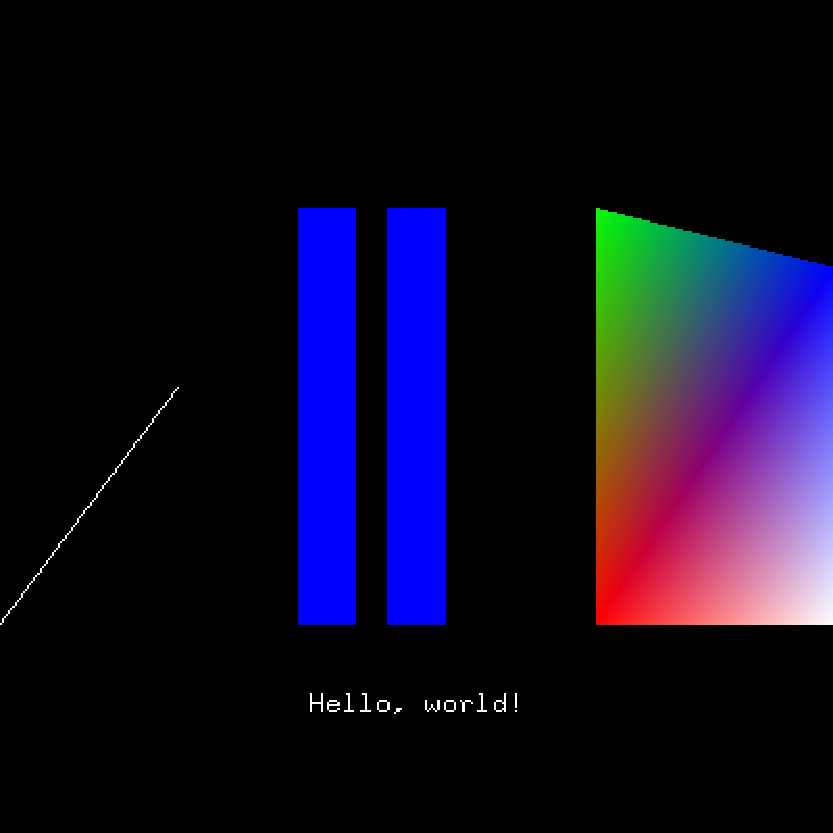
\includegraphics[height=3in]{figures/01_basics.pdf}
\end{center}
\caption{Screenshot of SUMMON with \code{examples/01\_basics.py}}
\label{fig:01_basics}
\end{figure}


\begin{figure}
\begin{center}
\begin{minipage}{6in}
{ \footnotesize
\begin{verbatim}
#!/usr/bin/env python-i
# SUMMON examples
# 01_basics.py - basic commands

# make summon commands available
from summon.core import *
import summon

# syntax of used summon functions
# add_group( <group> )   = adds a group of graphics to the screen
# group( <elements> )    = creates a group from several graphical elements
# lines( x1, y1, x2, y2, ... )  = an element that draws one or more lines
# quads( x1, y1, ..., x4, y4, ... )  = an element that draws one or more quadrilaterals
# color( <red>, <green>, <blue>, [alpha] ) = a primitive that specifies a color


# create a new window
win = summon.Window("01_basics")

# add a line from (0,0) to (30,40)
win.add_group(lines(0,0, 30,40))

# add two blue quadrilaterals inside a group
win.add_group(group(color(0, 0, 1), 
                    quads(50,0, 50,70, 60,70, 60,0),
                    quads(65,0, 65,70, 75,70, 75,0)))

# add a multi-colored quad, where each vertex has it own color
win.add_group(quads(color(1,0,0), 100, 0,
                    color(0,1,0), 100, 70,
                    color(0,0,1), 140, 60,
                    color(1,1,1), 140, 0))


# add some text below everything else
win.add_group(text("Hello, world!",     # text to appear
                   0, -10, 140, -100,   # bounding box of text
                   "center", "top"))    # justification of text in bounding box

# center the "camera" so that all shapes are in view
win.home()

\end{verbatim}
}
\end{minipage}
\end{center}
\caption{Source code for example/01\_basics.py}
\label{fig:01_basics_code}
\end{figure}

In your text editor, the example \code{01\_basics.py} should contain 
python code similar to \figref{fig:01_basics_code}.
The first two lines of the script import the SUMMON module \code{summon} and
all of  the basic SUMMON functions (\code{group}, \code{lines}, \code{color},
etc) from the \code{summon.core} module into the current environment.   A new
SUMMON graphics window is created using the \code{summon.Window} object.

All graphics are added and removed from the window in sets called {\em groups}. 
Groups provide a way to organize graphical elements into a hierarchy.
The first graphical group added to the window is a line.
The line is created with the \code{lines} function, which takes a series of
numbers specifying the end-point coordinates for the line.  The first
two numbers specify the x and y coordinates of one end-point (0,0) and the last
two specify the other end-point (30,40).  Next, the line is added to the window
using the \code{add\_group} function.

The next part of the example adds two quadrilaterals to the window with the
\code{quads} and \code{group} commands.  The arguments to the \code{quads}
function are similar to the \code{lines} function, except four vertices (8
numbers) are specified.  In the example, two quadrilaterals are created and
grouped together with the \code{group} function.

Note, both the \code{lines} and \code{quads} functions can draw multiple lines
and quadrilaterals (hence their plural names) by supplying more coordinates as
arguments.

The third group illustrates the use of color.  Color is stateful, as in OpenGL,
and all vertices that appear after a color object in a group will be affected. 
The \code{color} function creates a color object, which can appear
within graphical elements such as \code{lines} and \code{quads} or directly
inside a group.  Since each vertex in this example quad has a different color,
OpenGL will draw a quadrilateral that blends these colors.

Lastly, an example of text is shown.  Once again the text is added to the window
using the \code{add\_group} function.  The arguments to the \code{text} function
specify the text to be displayed, a bounding box specified by two
opposite  vertices, and then zero or more justifications ("left", "right",
"center", "top", "bottom", "middle") that will affect how the text aligns 
within its bounding box.  There are currently three types of text: \code{text}
(bitmap), \code{text\_scale} (stroke), \code{text\_clip} (stroked text that
clips).  The bitmap text will clip if it cannot fit within its bounding box. 
This is very useful in cases where the user zooms out very far and no more space
is available for the text to fit.  See the example \code{10\_text.py} for a
better illustration of the different text constructs.

The final function in the script is \code{win.home()}, which causes
the SUMMON window to scroll and zoom such that all graphics are visible.  This
is a very useful command for making sure that what you have drawn is visible in
the window.  The command can also be executed by pressing the 'h' key within a
SUMMON window.  This key  comes in handy when you "lose sight" of the
visualization.

This is only a simple example.  See the remaining scripts in the 
\code{summon/examples/} for examples of SUMMON's more powerful features.



\subsection{Example visualizations: SUMMATRIX and SUMTREE}

In the \code{summon/bin/} directory are two programs, \code{summatrix} and
\code{sumtree} that use SUMMON to visualize large datasets.  They are simply 
python scripts and so can be easily extended.  In my own work, I have 
extended the tree visualization program to integrate more closely with
biological data (executing CLUSTALW and MUSCLE on subtrees, displaying GO terms,
etc.).  Since these visualization programs are simply python scripts,
others can easily overlay and integrate their own data.  

Also in both visualizations the underling data is accessible through global
python variables.  That means if you have a very specific question like, ``How
many genes in my subtree have a particular GO term?'', you can quickly write a
few lines of python to walk the tree and answer the question yourself.  It would
be very difficult to anticipate all such questions during the development of a
non-scriptable visualization.

Example input files for both programs can be found under the 
\code{summon/examples/summatrix/} and \code{summon/examples/sumtree/}
directories. Both programs will print their usage if run with no arguments. 
View/execute the \code{view\_*.sh} scripts for examples of how to call
\code{summatrix} and  \code{sumtree}.


%\comment{
%=============================================================================
\section{SUMMON Features}

\subsection{The SUMMON Window}
    
Each window opened by SUMMON is an instantiation of the \code{summon.Window}
class. This class provides the interface to manipulate the window (title, size,
position, etc.) as well as to manipulate the graphical elements it  displays
(\code{add\_group}, \code{remove\_group}, etc.).  

\subsection{Models}

Each window is associated with two models (see \code{Model} class), called the
\code{world} and \code{screen} which are accessible as \code{Window.world} and
\code{Window.screen}.  A model contains drawing elements such as lines, and
polygons.  The units of the world model's coordinate system  can
be whatever the user wants, provided that the x- and y- axis increase to 
the right and top, respectively.   The size and orientation of the world 
model is dependent on scrolling and zooming. The world model is the
default model that is  used when drawing (e.g. functions such as
\code{Window.add\_group} forward their arguments to 
\code{Window.world.add\_group}).

In contrast, the screen model is always drawn with its origin at the 
lower left corner of the window and with units in terms of pixels. The
screen model is always drawn on top of the world model.  The screen model
is often used to draw menus, toolbars, or other things that should always
be in view, and should not be affected by scrolling and zooming.
%}



%=============================================================================
\section{SUMMATRIX: large-scale sparse matrix visualizer}

SUMMATRIX is a visualization for matrices (\figref{fig:summatrix}) built with
SUMMON.  It can be executed either from the command-line with the supplied demo
(\code{summatrix}) or  instantiated as an object
(\code{summon.matrix.MatrixViewer}) from within your own python program. 
SUMMATRIX also includes support for visualizing data clustering and other
matrix permutations.  To see all of SUMMATRIX's options run \code{summatrix} on
the command-line with no options.  Examples of using SUMMATRIX can be found in
the \code{summon/examples/summatrix/} directory.


%============================
\begin{figure}
\begin{center}
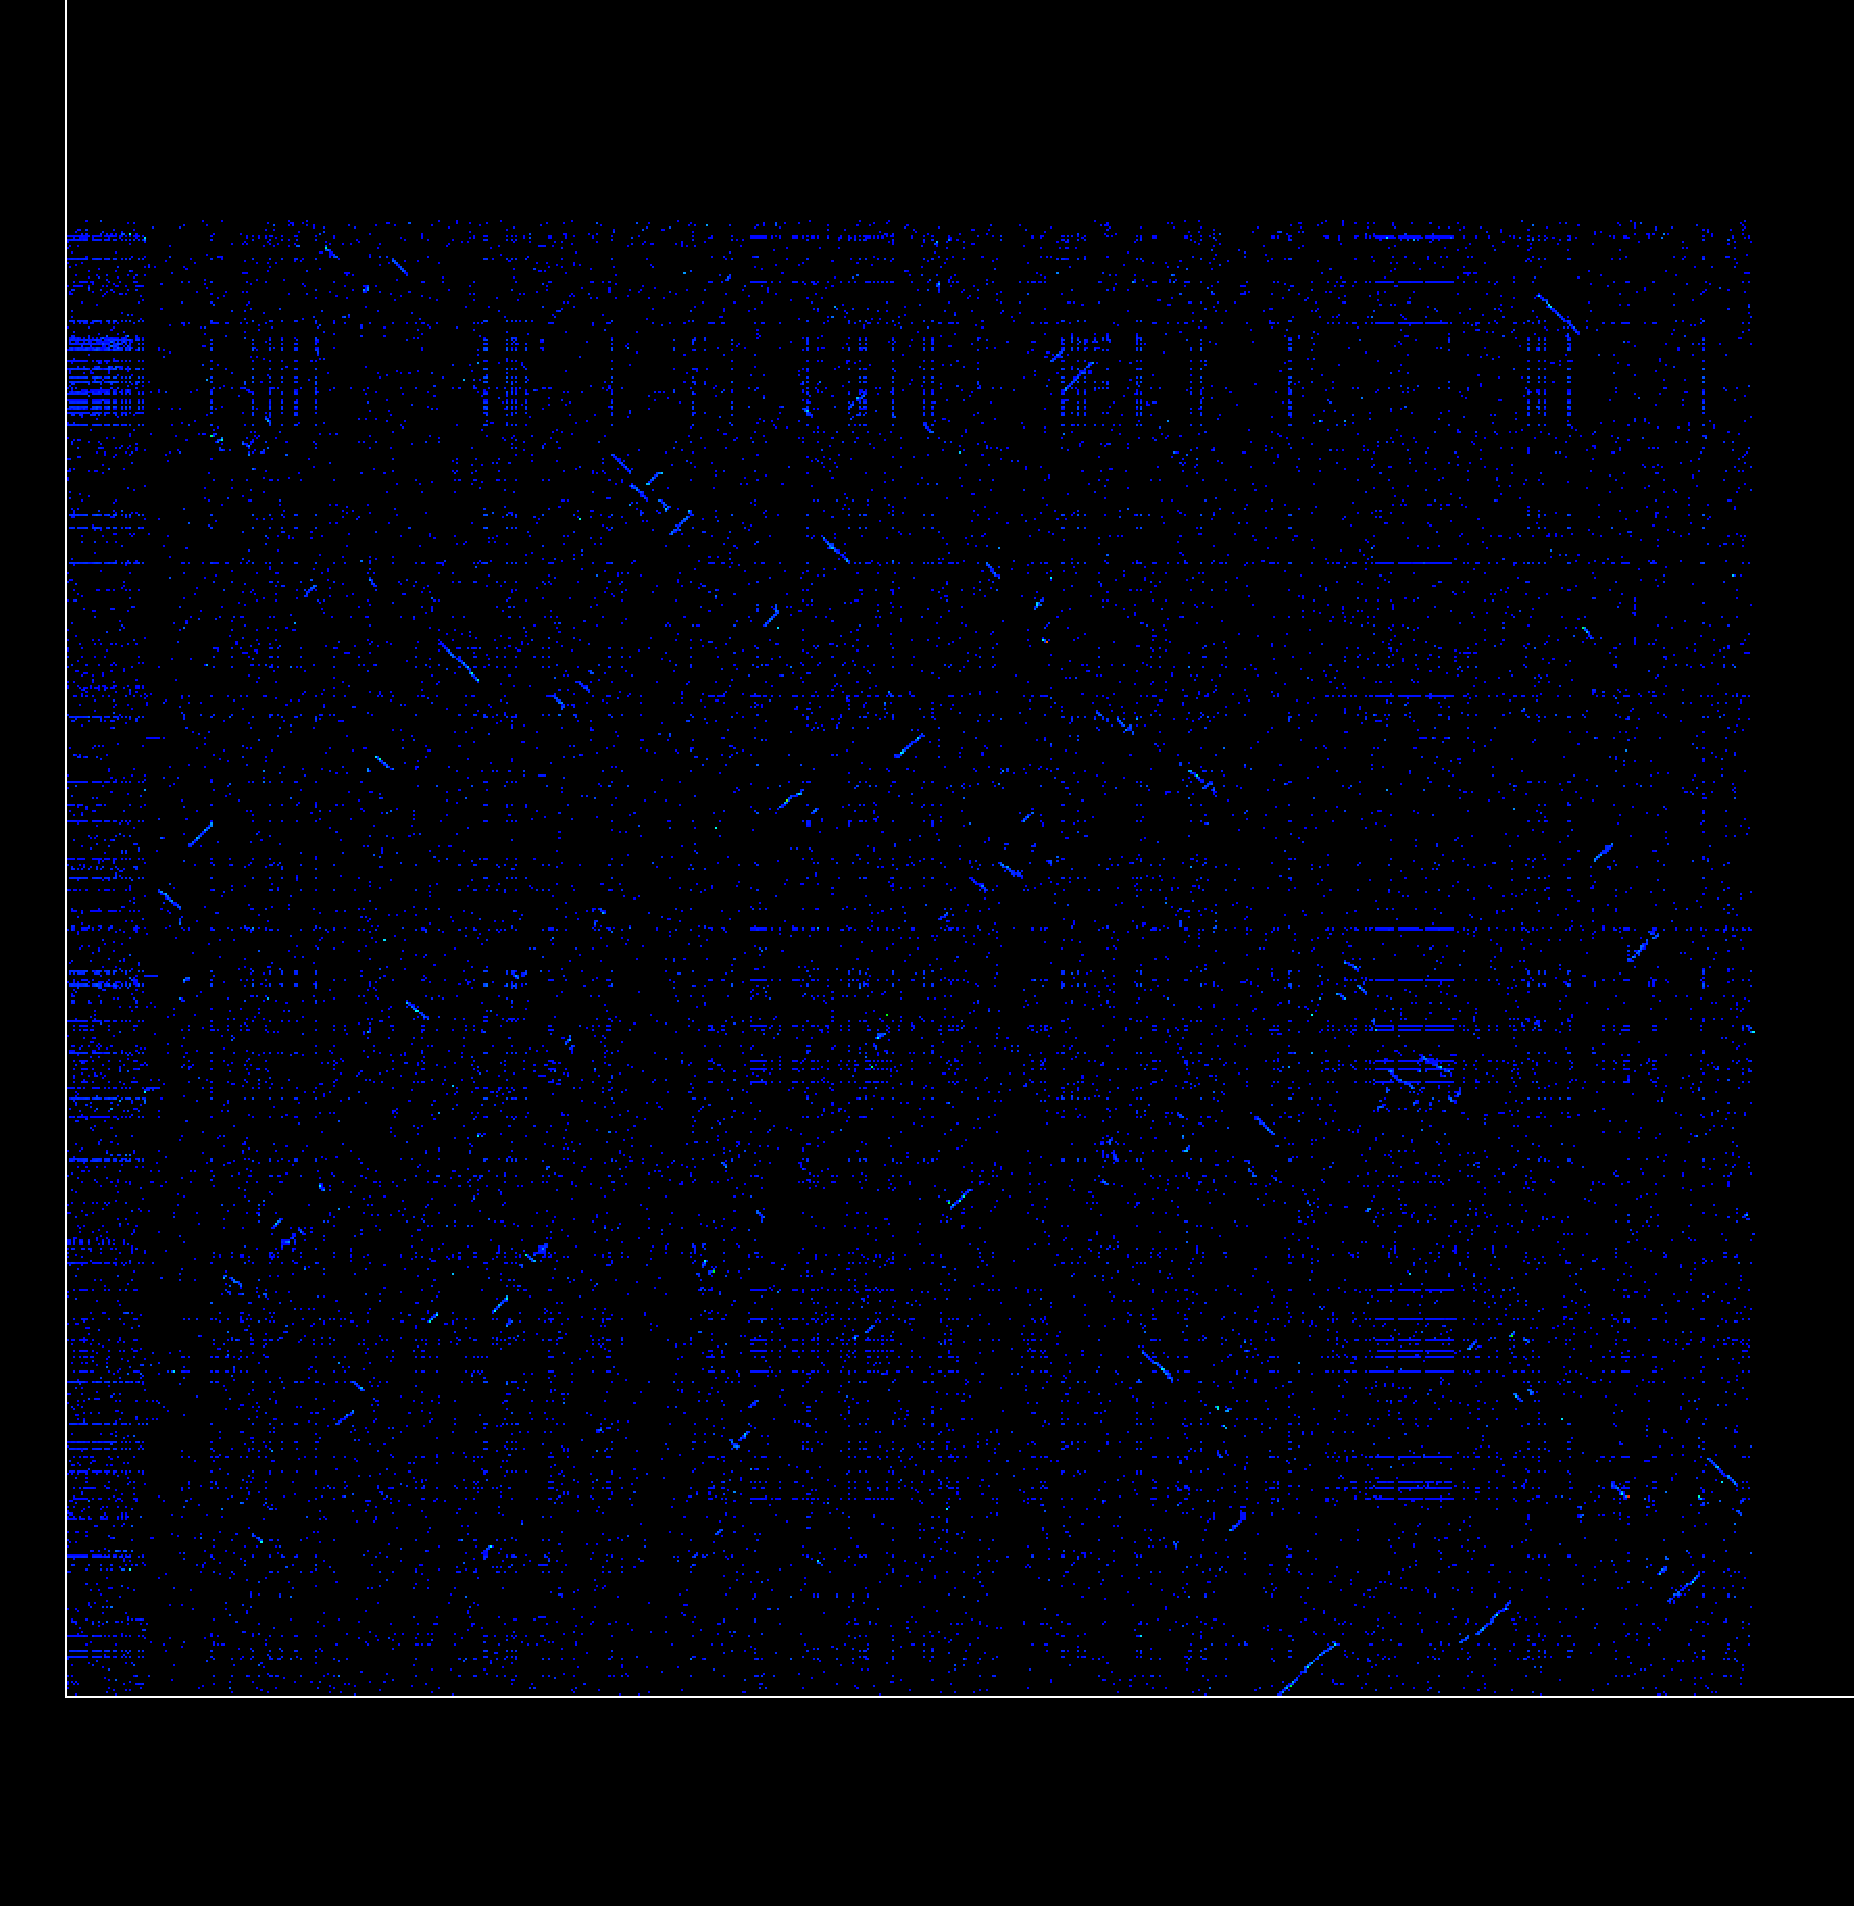
\includegraphics[height=3in]{figures/summatrix.pdf}
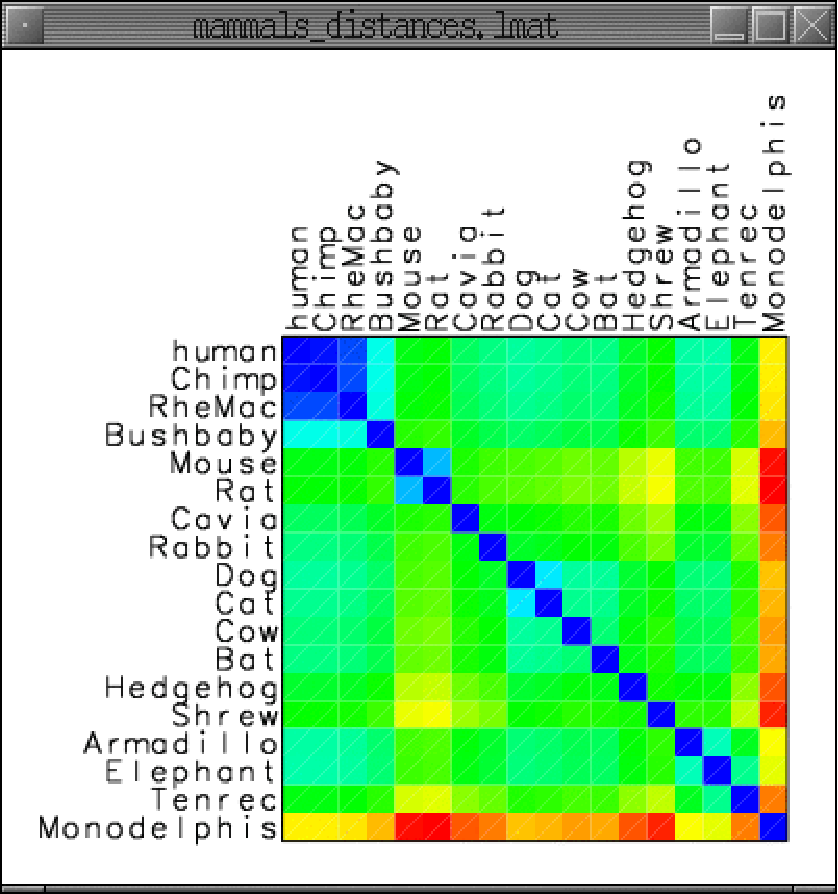
\includegraphics[width=3in,height=3in]{figures/summatrix-mammals.pdf}
\end{center}
\caption{Example screenshots of SUMMATRIX on both sparse and dense matrices}
\label{fig:summatrix}
\end{figure}


\subsection{Matrix file formats}

\code{summatrix} visualizes dense and sparse matrices stored in a variety of 
formats.

\begin{itemize}

    %============================================================
    \item {\bf dense format.}
    The {\em dense matrix format} is for small matrices with many non-zero entries.
    The first line of a {\em dense matrix file} (\code{*.mat})
    contains two white-space delimited integers:
    
    \codeblock{nrows ncols}
    
    where \code{nrows} and \code{ncols} are the number of rows and columns in
    the matrix.  The remaining \code{nrows} lines of
    the file specify each row of the matrix with \code{ncols} white-space
    delimited numbers (integer or float).  For example:

    \codeblock{val1 val2 val3 ... valN}

    \code{summatrix} will load a {\em dense matrix} with the \code{-d}
    and  \code{--dense} options.
    
    See \code{examples/summatrix/clustering/data.mat} for an example.
    
    
    %=============================================================
    \item {\bf compressed row format (sparse).}
    The {\em compressed row format} is for large matrices with only a
    relatively few non-zero entries.
    The first line of a {\em compressed row matrix file} (\code{*.mat})
    contains three white-space delimited integers:
    
    \codeblock{nrows ncols nnz}
    
    where \code{nrows} is the number of rows, \code{ncols} is the number of
    columns, and \code{nnz} is the total number of non-zero entries in the
    matrix.  The remaining \code{nrows} lines of the file specify each row of
    the matrix in the following format:

    \codeblock{col1 val1 col2 val2 col3 val3 ...}

    which indicates that for this $row$ of the matrix we have
    
    \codeblock{
        matrix[row][col1] = val1 \newline
        matrix[row][col2] = val2 \newline
        matrix[row][col3] = val3 \newline
        ... 
    }
    
    
    Note that \code{colN} is an integer and 1-based (1st column is
    numbered 1, last column is numbered $ncols$) and \code{valN} can be a 
    float or integer.  Any entry of the matrix not specified is assumed to be
    zero.

    \code{summatrix} will load a {\em compressed row matrix} with the \code{-r}
    and  \code{--rmat} options.
    
    See \code{examples/summatrix/dog\_human.mat} for an example.


    %=============================================================
    \item {\bf index format (sparse).}
    The {\em index format} is for large matrices with only a
    relatively few non-zero entries.     
    The first line of an {\em index matrix file} (\code{*.imat}) contains three
    white-space delimited integers:
    
    \codeblock{nrows ncols nnz}
    
    where \code{nrows} is the number of rows, \code{ncols} is the number of
    columns, and \code{nnz} is the total number of non-zero entries.  The
    remaining \code{nnz} lines of  the file specify each non-zero entry with the
    format:

    \codeblock{row col val}

    which indicates that $matrix[row][col] = val$.  Note that 
    \code{row} and \code{col} are integers and 0-based (1st row and column are
    numbered 0, last row and column are numbered $nrows-1$ and $ncols-1$,
    respectively) and \code{val} can be a float or integer.  Any entry of the
    matrix not specified is assumed to be zero.

    \code{summatrix} will load an {\em index matrix} with the \code{-i} and 
    \code{--imat} options.
    
    See \code{examples/summatrix/human\_mouse.imat} for an example.


    %==============================================================
    \item {\bf labeled format (sparse).}       
    This format is similar to {\em index format} except instead of specifying
    row and column by an integer, they are specified by a unique string 
    ({\em label}).
    The total number of rows, columns, and non-zeros does not need to be
    specified. Instead each line of the file has the following format:

    \codeblock{rowlabel collabel val}

    which indicates that $matrix[rowlabel][collabel] = val$.  Note that 
    \code{row} and \code{col} are strings and \code{val} can be a float or 
    integer.  Rows and columns are drawn in the order (left-to-right,
    top-to-bottom) that are first mentioned in the file.  
    A different ordering can specified with the \code{--order} option and a file
    containing the labels in the desired order, one label per line.
    Any entry of the matrix not specified is assumed to be zero.
    
    \code{summatrix} will load a {\em labeled matrix} with the \code{-l} and 
    \code{--lmat} options.
    
    See \code{examples/summatrix/mammals\_distances.lmat} for an example.

\end{itemize}


\subsection{Row and column label formats}

SUMMATRIX can display row and column labels.  They are specified with the 
\code{--rlab=$filename$} and \code{--clab=$filename$} command-line options.  If
your matrix is square and the row and column labels are the same, you can
specify them with only one option using \code{--rclab=$filename$}.  The label
file format is simple a text file with one label per line in the order that the
rows (or columns) appear in the matrix.

Labels will be used when the user clicks on an entry in the matrix.  Labels can
also be displayed on the sides of the matrix with the \code{--showlabels} option
or by pressing the ``l'' key during visualization.  The \code{inline} option
will draw the labels in the same window as the matrix.  The \code{panels} option
will draw the labels in neighboring windows, such that the labels are never out
of view while zooming and scrolling.



\subsection{Visualizing data clustering}

SUMMATRIX allows easy visualization of clustering.  However, you must use
another  third-party program to actually cluster your data.  If you are looking
for ideas, I recommend taking a look at the CLUTO clustering toolkit at 
\code{http://glaros.dtc.umn.edu/gkhome/views/cluto}.  Many of the file formats
used by SUMMON are compatiable with this software package.

\subsubsection{Row and column permutation}

Using such a clustering program you can visualize your clustering as a
permutation of the rows (or columns) of your data matrix.  SUMMATRIX will
permute your matrix if you specify any of the options 
\code{--rperm=$filename$}, \code{--cperm=$filename$}, or 
\code{--rcperm=$filename$}.  Where $filename$ is a permutation file, which is a
text file with $nrows$ (or $ncols$) lines with one integer per line. 
The integer indicates which row (or column) should appear in this position. The
integer is 0-based (1st row is 0, last is $nrows-1$).

See \code{examples/summatrix/clustering/data.rperm} for an example of a
row permutation file.

\subsubsection{Row and column partitioning}

SUMMATRIX can also draw horizontal and vertical lines that divide the matrix
into sub-divisions that represent your clusters.  This is done with the 
\code{--rpart=$filename$}, \code{--cpart=$filename$}, and
\code{--rcpart=$filename$} options.  The file $filename$ should be in the 
{\em partition format}, which is a text file with $nrows$ (or $ncols$) lines
with one string per line.  Each string indicates the cluster of the
corresponding row (or column).  For example, if your matrix is clustered by
rows into three clusters called ``ClusterA'', ``ClusterB'', and ``ClusterC'',
then those three strings should used in the partition file.  Clusters can also
be named with integers as in the supplied example.

See \code{examples/summatrix/clustering/data.rpart} for an example of a
row partition file.

If a permutation file is specified the matrix will be permuted, and dividers
will be drawn when ever two neighboring rows (or columns) are associated with
different clusters.  If no permutation file is given, the rows (or columns) will
be sorted automatically by their cluster label.

\subsubsection{Row and column hierarchical trees}

%============================
\begin{figure}
\begin{center}
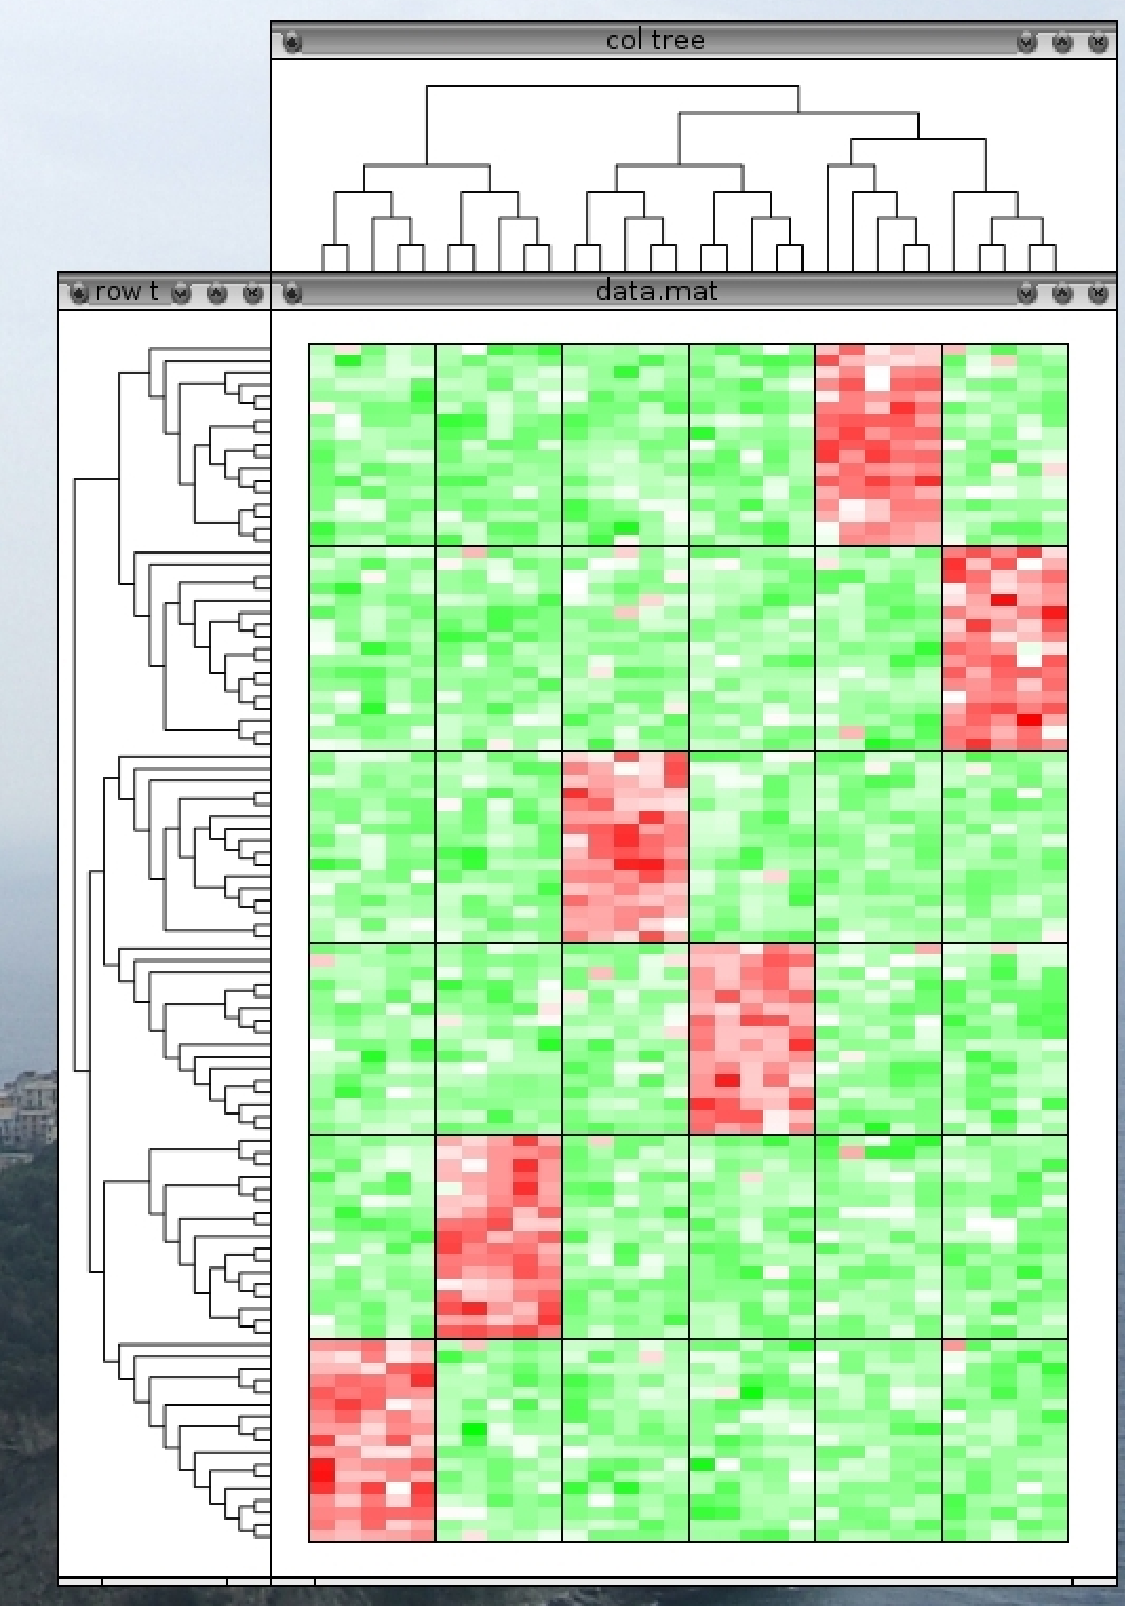
\includegraphics[width=2in]{figures/summatrix-trees.pdf}
\end{center}
\caption{Example of row and column hierarchical trees in SUMMATRIX can 
be used to visualize a clustering.  Cluster partions (black horizontal and
vertical lines) are shown with \code{--rpart,cpart} and trees are specified with
\code{--rptree,--cptree}. 
See  \code{examples/summatrix/clustering/view\_data\_tree\_clustered.sh}}
\label{fig:summatrix_trees}
\end{figure}


SUMMATRIX supports displaying hierarchical trees next to a matrix 
(\figref{fig:summatrix_trees}), which is often useful for visualizaling
a clustering.  
Trees are specified with the following options.

\code{
  --rptree <row parent tree file>

  --cptree <column parent tree file>

  --rtree <row tree newick file>

  --ctree <column tree newick file>  
}

When a tree is specified it will be displayed in a separate window aligned next
to the matrix.  The rows (or columns) of the matrix will be permuted to match
the order of the leaves in the tree.  If a permutation file is given
(\code{--rperm,--cperm}) it is ignored.

Two tree file formats are currently supported: ptree and newick.  See
\secref{sec:sumtree} for a description of the formats.
If you use the ptree format (\code{--rptree,--cptree}) the leaves should be 
numbered with the same index as its corresponding row (or column) in the 
matrix.  If you use the newick format (\code{--rtree,--ctree}) the leaves should
either be integers corresponding to the rows (or columns) of the matrix, or 
be strings that match the row (column) labels of the matrix
(\code{--rlab,--clab}).
    
See \code{examples/summatrix/clustering/data.row.ptree} for an example of a
ptree for a clustered matrix.
   


%=============================================================================
\section{SUMTREE: large-scale tree visualizer}
\label{sec:sumtree}

SUMTREE is a visualization for trees built on top of the SUMMON library.  It can
be executed either from the command-line with the supplied demo (\code{sumtree})
or  instantiated as an object (\code{summon.sumtree.SubTree}) from within your
own python program.  SUMTREE is useful for visualizing trees from hierarchical
clusterings or phylogenetic reconstructions.  To see all of SUMTREE's options
run \code{sumtree} on the command-line with no options.  Examples of using
SUMTREE can be found in the \code{summon/examples/sumtree/} directory.

%============================
\begin{figure}
\begin{center}
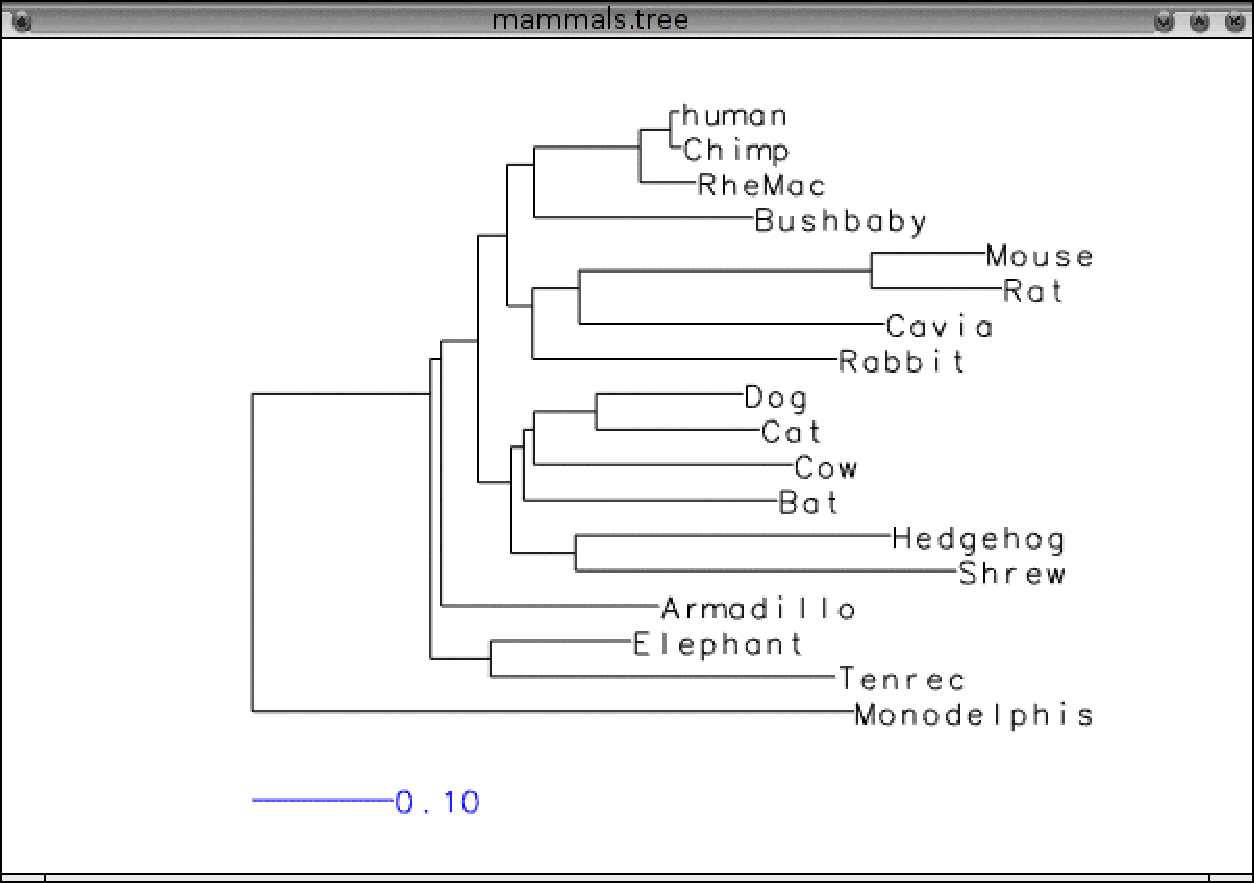
\includegraphics[width=3in]{figures/sumtree-mammals.pdf}
\end{center}
\caption{Example of a phylogenetic tree visualized with SUMTREE.
See  \code{examples/sumtree/view\_mammals.sh}}
\label{fig:sumtree}
\end{figure}

\subsection{Tree file formats}

SUMTREE currently supports two file formats:

\begin{itemize}

    \item {\bf ptree format.}
    The {\em ptree} (parent tree) format is a simple format that is also produced by the
    CLUTO clustering package.  It specifies a binary tree of $n$ leaves by assigning
    each node in the tree an integer.  The leaves are numbered $0$ to $n-1$, the
    internal nodes are numbered $n-2$ to $2n-3$, and the root is
    numbered $2n-2$.  The ptree file contains a list of
    $2n-1$ integers, one integer per line.  The line $i$ (0-based) should contain
    the id-number of the {\em parent} of node $i$.  The last line (line $2n-2$) 
    should contain the integer -1 to indicate that the root of the tree has no
    parent.  See 
    \code{examples/summatrix/clustering/data.row.ptree} and
    \code{examples/sumtree/dog-human-genes.ptree} for examples.

    
    \item {\bf newick format.}
    The {\em newick} format is a standard format commonly used for storing
    phylogenetic trees \url{http://en.wikipedia.org/wiki/Newick_format}.  The
    structure of the tree is specified with a parenthesis notation.  For example a
    five leaf tree with leaves named A, B, C, D, and E can be written in Newick as:

    \code{(((A,B),(C,D)),E);}

    This states that A and B are sisters, C and D are sisters, A and C are cousins,
    and E is a great uncle of A.

    Branch lengths can also be specified by adding a
    colon followed by a floating point number the end of any node in the tree.

    \code{(((A:1,B:2):1.5,(C:0.5,D:0.2):1.2):3,E:6);}

    For example, the above states that the branch directly above A is length 1 and
    the branch directly above C is 0.5.  Also note that the internal node branch 
    lengths are also given (e.g. the length of the branch directly above the
    parent of A is 1.5).

\end{itemize}

%=============================================================================
\section{SUMMON function reference}

See \code{summon.html} for complete function reference.

\end{document}
